\chapter{Observability and Consistency of VIO}
\label{ch:observability}
\chaptermark{Observability and Consistency} % short running header

\begin{objectives}
\begin{itemize}
  \item Define observability for nonlinear systems, and test it with Lie derivatives.
  \item Prove that VIO has four unobservable directions and write them in the project's error coordinates.
  \item Show, in the planar EKF-SLAM problem where every step can be computed, exactly how the standard EKF acquires spurious information,
        and see it happen in a Monte Carlo simulation.
  \item Prove that First-Estimates Jacobians restore the correct unobservable subspace, and understand the alternatives: the
        observability-constrained EKF, the invariant EKF and robocentric formulations.
  \item Know the degenerate motions that remove further information.
\end{itemize}
\end{objectives}

The planar MSCKF of \cref{ch:planar} was consistent, but its NEES crept upward. This chapter explains the creep. The explanation needs one
new idea, observability, and one careful computation, the observability matrix of a linearized filter. The computation is done in full for
planar EKF-SLAM, the setting in which the effect was first understood~\cite{julier2001counter, bailey2006consistency, huang2010observability},
and then carried over to VIO.

% ------------------------------------------------------------------------------
\section{Observability}

\subsection{Indistinguishable states}

Consider a system $\dot x = f(x, u)$ with output $y = h(x)$. Two initial states $x_0$ and $x_0'$ are \term{indistinguishable} if, for every input
signal $u(\cdot)$, they produce the same output signal $y(\cdot)$. No estimator, however clever, can tell them apart: the data are identical. A
system is \emph{observable} at $x_0$ if no other state is indistinguishable from it. Since estimators work locally, the useful notion is
local: $x_0$ is \termi{locally weakly observable}{observability!local weak} if it can be distinguished, over arbitrarily short time intervals, from
every state in some neighborhood of it.

For linear systems the question is settled by the observability matrix (\cref{thm:obs-rank}). For a time-varying linear system
$\delta x_{k+1} = \Phi_k\delta x_k$, $r_k = H_k\delta x_k$ the same object reads as follows.

\begin{definition}[Observability matrix]
\label{def:obs-matrix}
The observability matrix over steps $1, \dots, k$ is
\begin{equation}
  \mathcal{O} = \begin{bmatrix} H_1 \\ H_2\Phi_1 \\ H_3\Phi_2\Phi_1 \\ \vdots \\ H_k\Phi_{k-1}\cdots\Phi_1 \end{bmatrix}.
\end{equation}
An initial error $\delta x_1 \in \nullsp(\mathcal{O})$ produces no change in any measurement, so it cannot be detected.
$\nullsp(\mathcal{O})$ is the \term{unobservable subspace}.
\end{definition}

A Kalman filter can gain information only in directions outside $\nullsp(\mathcal{O})$. Along unobservable directions its covariance may grow
(from process noise) but must never shrink. This is the property that the standard EKF violates.

\subsection{Nonlinear observability and Lie derivatives}

For a nonlinear system the observability matrix is replaced by derivatives of the output along the dynamics. Suppose the dynamics are
\emph{control-affine}, $\dot x = f_0(x) + \sum_i f_i(x)\,u_i$, as kinematic models usually are (the inputs are the measured rates and
accelerations). The \termi{Lie derivative}{Lie derivative} of a scalar function $\varphi$ along a vector field $f$ is its rate of change along the flow of $f$,
\begin{equation}
  L_f\varphi(x) = \nabla\varphi(x)\cdot f(x),
\end{equation}
and repeated derivatives are written $L_gL_f\varphi = \nabla(L_f\varphi)\cdot g$. Differentiating the output along a trajectory gives
\begin{equation}
  y = h(x), \qquad \dot y = L_{f_0}h + \sum_i u_i\,L_{f_i}h, \qquad \ddot y = \dots
\end{equation}
Because the inputs can be varied freely, each Lie derivative $L_{f_i}h$ is, in effect, a separate measured function of the state, and so are
the higher ones. If enough of them are available, their values pin down the state.

\begin{theorem}[Observability rank condition~\cite{hermann1977nonlinear}]
\label{thm:obs-rank-nonlinear}
Let $d\mathcal{O}(x)$ be the span of the gradients of $h$ and of all its repeated Lie derivatives $L_{f_{i_1}}\cdots L_{f_{i_m}}h$ along the vector fields of
the system. If $\dim d\mathcal{O}(x_0) = n$, the system is locally weakly observable at $x_0$.
\end{theorem}
\begin{proof}[Idea of the proof]
Choose $n$ of the functions whose gradients are independent at $x_0$ and stack them into $\Psi(x) \in \R^n$. Each is determined by the output
and the inputs (by differentiation), and $\Psi$ has an invertible Jacobian at $x_0$, so by the inverse function theorem it is one-to-one near $x_0$.
Two nearby states with the same outputs would have the same $\Psi$, hence coincide.
\end{proof}

For a linear system, $f_0 = Ax$ and $h = Cx$, the gradients are $C, CA, CA^2, \dots$: the rank condition is \cref{thm:obs-rank}. For analytic systems the
condition is also necessary in a generic sense, so a rank deficiency at typical states signals a genuine family of indistinguishable states.

\begin{worked}[a planar robot and a landmark]
A planar robot (\cref{ch:planar}) with pose $(p, \psi)$ measures the position of a landmark $\ell$ in its body frame, $h = R(\psi)\T(\ell - p) \in \R^2$. Its kinematics
are $\dot p = R(\psi)e_1\,v$ and $\dot\psi = \omega$, that is $f_v = (R(\psi)e_1, 0)$ and $f_\omega = (0, 1)$ with inputs $v$ and $\omega$.

\emph{Unknown landmark.} The state is $x = (p, \psi, \ell) \in \R^5$. With $\partial(R\T a)/\partial\psi = -\Omega R\T a$ (\cref{lem:omega}),
\begin{equation*}
  \nabla h = \begin{bmatrix} -R\T & -\Omega h & R\T \end{bmatrix}, \qquad
  L_{f_v}h = -R\T Re_1 = -e_1, \qquad L_{f_\omega}h = -\Omega h .
\end{equation*}
The first Lie derivative is constant (its gradient is zero), and $\nabla(L_{f_\omega}h) = -\Omega\nabla h$ has the same row space as $\nabla h$. Every further
derivative repeats the pattern, so $\dim d\mathcal{O} = 2$: three of the five directions are unobservable. They are the two global translations and the
global rotation, exactly the directions of \cref{sec:planar-unobservable}.

\emph{Known landmark.} If $\ell$ is known, $x = (p, \psi) \in \R^3$, the gradients are $[-R\T\ \ {-\Omega h}]$ and its multiples by $\Omega$, and the rank is 2: one
direction is unobservable. It is the rotation of the robot about the landmark, which leaves the body-frame landmark position unchanged. One known
landmark fixes position but not heading; two fix both.
\end{worked}

% ------------------------------------------------------------------------------
\section{The four unobservable directions of VIO}
\index{unobservable directions!VIO}

\begin{theorem}[Unobservable directions of VIO]
\label{thm:vio-unobservable}
For monocular VIO with point features, applying the same global translation $t$ and the same rotation $R_z(\alpha)$ about the
gravity direction to all positions, velocities, attitudes, clones and features leaves every IMU and camera measurement
unchanged. The state is therefore unobservable along these four directions.
\end{theorem}
\begin{proof}
Under $p \mapsto R_zp + t$, $v \mapsto R_zv$, $R_{wb} \mapsto R_zR_{wb}$, $p_f \mapsto R_zp_f + t$, with biases unchanged:
\begin{itemize}
  \item the gyroscope measures $\sx{\omega_b} = R_{wb}\T\dot R_{wb}$, which is invariant because $R_z$ is constant;
  \item the accelerometer measures $R_{wb}\T R_z\T(R_za_w - g_w) = R_{wb}\T(a_w - R_z\T g_w) = R_{wb}\T(a_w - g_w)$, because a rotation about
        gravity leaves $g_w$ unchanged;
  \item the camera sees $R_{bc}\T\big(R_{wb}\T R_z\T(R_zp_f + t - R_zp - t) - p_{bc}\big) = R_{bc}\T\big(R_{wb}\T(p_f - p) - p_{bc}\big)$.
\end{itemize}
All measurements are identical, so the transformed and original trajectories cannot be distinguished.
\end{proof}

Rotations about horizontal axes are \emph{not} in this family, because they would rotate gravity in the accelerometer equation;
roll and pitch are observable. Scaling is not either, because it would scale the accelerations the accelerometer measures;
scale is observable as long as the vehicle accelerates. That the remaining directions (velocity, roll, pitch, scale, biases) \emph{are}
observable under general motion is proved with the rank condition of \cref{thm:obs-rank-nonlinear}; see~\cite{hesch2014consistency} for the
computation.

Linearizing the transformation gives the unobservable directions in the project's error coordinates. With $e_z$ the vertical
unit vector, a small yaw rotation $\alpha$ and a small translation $t$ change the state by (verified numerically):
\begin{equation}
  \underbrace{\begin{bmatrix} \delta p \\ \delta v \\ \delta\theta \\ \delta b_a \\ \delta b_g \\ \delta p_i \\ \delta\theta_i \\ \delta p_f \end{bmatrix}}_{\text{error state}}
  = \underbrace{\begin{bmatrix}
    I_3 & -\sx{\hat p}\,e_z \\
    0 & -\sx{\hat v}\,e_z \\
    0 & \hat R\T e_z \\
    0 & 0 \\
    0 & 0 \\
    I_3 & -\sx{\hat p_i}\,e_z \\
    0 & \hat R_i\T e_z \\
    I_3 & -\sx{\hat p_f}\,e_z
  \end{bmatrix}}_{N}
  \begin{bmatrix} t \\ \alpha \end{bmatrix}.
  \label{eq:nullspace-N}
\end{equation}
The last row applies only to formulations that keep features in the state. The position entries follow from
$R_z(\alpha)p \approx p + \alpha\,e_z\times p = p - \alpha\sx{p}e_z$; the attitude entry is $\hat R\T e_z$ because the error is
local: $\Exp(\alpha e_z)\hat R = \hat R\,\Exp(\alpha\hat R\T e_z)$, a rotation about the world vertical expressed in body axes. Every column of $N$ \emph{depends on
the estimate}: the yaw column involves $\hat p$, $\hat v$, $\hat R$ and the clone and feature estimates. That dependence is the root of the problem.
\Cref{eq:planar-nullspace} is the planar version, with $\Omega\hat p$ in place of $-\sx{\hat p}e_z$.

% ------------------------------------------------------------------------------
\section{Why the standard EKF becomes overconfident}

If every Jacobian were evaluated at the true state, the linearized system would satisfy $\mathcal{O}N = 0$ at all times, and the
filter would never gain information along $N$. The EKF instead evaluates each Jacobian at the best estimate available when it is
computed. The transition matrix $\Phi_k$ is evaluated at the estimate after the update at step $k$, while the measurement Jacobian at step $k$ was evaluated
at the estimate before that update. The same physical state enters the observability matrix linearized at two different points, and the products
$H_k\Phi_{k-1}\cdots\Phi_1N$ no longer cancel. The planar EKF-SLAM problem shows this in a computation short enough to do completely.

\subsection{Planar EKF-SLAM}
\index{EKF-SLAM!inconsistency}\index{inconsistency!EKF}

The state is the robot pose and $L$ landmarks, $x = (p, \psi, \ell_1, \dots, \ell_L)$, with additive errors. Odometry propagates the robot
($p_{k+1} = p_k + R(\psi_k)e_1v_m\Dt$, $\psi_{k+1} = \psi_k + \omega_m\Dt$), landmarks are static, and an observation of landmark $j$ is its position in the
body frame, $z = R(\psi)\T(\ell_j - p) + n$. Writing $\hat x_{k|k-1}$ for the propagated estimate at step $k$ and $\hat x_{k|k}$ for the updated one, the EKF uses
\begin{align}
  \Phi_k &= \begin{bmatrix} I_2 & \Omega\,(\hat p_{k+1|k} - \hat p_{k|k}) \\ 0 & 1 \end{bmatrix} \oplus I_{2L}, \label{eq:slam-phi} \\
  H_k &= \begin{bmatrix} -\hat R_k\T & -\Omega\hat R_k\T(\hat\ell_j - \hat p_{k|k-1}) & 0 \cdots 0 & \hat R_k\T & 0 \cdots 0 \end{bmatrix},
  \qquad \hat R_k = R(\hat\psi_{k|k-1}), \label{eq:slam-H}
\end{align}
where $\Phi_k$ follows from \cref{prop:planar-phi} (the step starts from the updated estimate), $H_k$ from the derivation of \cref{prop:planar-H} without the
projection, and $\hat\ell_j$ is the landmark estimate at the time of the update. The candidate unobservable directions, by the argument of
\cref{sec:planar-unobservable}, are the translations $N_t = (I_2, 0, I_2, \dots, I_2)$ and the rotation
\begin{equation}
  N_r(\bar p, \bar\ell) = \big(\Omega\bar p,\ 1,\ \Omega\bar\ell_1,\ \dots,\ \Omega\bar\ell_L\big),
\end{equation}
built from some reference values $\bar p$, $\bar\ell_j$ of the positions.

\begin{theorem}[Observability of linearized planar EKF-SLAM]
\label{thm:slam-obs}
Let $\Delta_i = \hat p_{i|i} - \hat p_{i|i-1}$ be the correction of the robot position by the update at step $i$, and $D_k = \sum_{i=1}^{k-1}\Delta_i$ (with $D_1 = 0$).
For every $k$, $H_k\Phi_{k-1}\cdots\Phi_1N_t = 0$, while
\begin{equation}
  H_k\Phi_{k-1}\cdots\Phi_1\,N_r(\hat p_{1|0}, \bar\ell) = \hat R_k\T\,\Omega\,\big(D_k + \bar\ell_j - \hat\ell_j\big).
  \label{eq:slam-leak}
\end{equation}
\end{theorem}
\begin{proof}
Each $\Phi_i$ is the identity plus a term in the heading column, so the product is
$\Phi_{k-1}\cdots\Phi_1 = \begin{bmatrix} I & \Omega\,s_k \\ 0 & 1\end{bmatrix} \oplus I$ with
\begin{equation*}
  s_k = \sum_{i=1}^{k-1}\big(\hat p_{i+1|i} - \hat p_{i|i}\big)
      = \sum_{i=1}^{k-1}\big(\hat p_{i+1|i} - \hat p_{i|i-1}\big) - \sum_{i=1}^{k-1}\big(\hat p_{i|i} - \hat p_{i|i-1}\big)
      = \hat p_{k|k-1} - \hat p_{1|0} - D_k ,
\end{equation*}
since the first sum telescopes. Translations: the product leaves $N_t$ unchanged and $H_kN_t = -\hat R_k\T + \hat R_k\T = 0$. Rotation: the product
maps the robot entries $(\Omega\hat p_{1|0}, 1)$ to $(\Omega\hat p_{1|0} + \Omega s_k, 1) = (\Omega(\hat p_{k|k-1} - D_k), 1)$ and leaves the landmark entries alone, so
\begin{equation*}
  H_k(\cdot) = -\hat R_k\T\Omega(\hat p_{k|k-1} - D_k) - \Omega\hat R_k\T(\hat\ell_j - \hat p_{k|k-1}) + \hat R_k\T\Omega\bar\ell_j
  = \hat R_k\T\Omega\big(D_k + \bar\ell_j - \hat\ell_j\big),
\end{equation*}
using $\hat R_k\T\Omega = \Omega\hat R_k\T$; the $\hat p_{k|k-1}$ terms cancel.
\end{proof}

\Cref{eq:slam-leak} is the whole story. The rotation direction stays in the nullspace only if two things vanish:
\begin{itemize}
  \item $D_k$, the accumulated corrections of the robot position. They vanish only if the transition matrices telescope, which requires each $\Phi_i$
        to start where the previous one ended. The EKF starts each $\Phi_i$ from the \emph{updated} estimate $\hat p_{i|i}$, while the previous one ended at the
        \emph{propagated} estimate $\hat p_{i|i-1}$.
  \item $\bar\ell_j - \hat\ell_j$, the change of the landmark estimate between its linearization points. A single fixed reference $\bar\ell_j$ cannot match an
        estimate that every update moves.
\end{itemize}
For generic estimates no other choice of reference values makes \eqref{eq:slam-leak} vanish for all $k$, and the unobservable subspace of the EKF's
linearized model shrinks from three dimensions to two~\cite{huang2010observability}: the heading has become observable. The filter then extracts
\emph{spurious information} about the global heading from measurements that contain none. The size of the leak is set by the size of the
corrections and of the landmark estimate changes; it is largest at loop closures, when a robot that has drifted re-observes old landmarks
and receives large corrections.

\subsection{From planar SLAM to VIO}

The same mechanism operates in VIO. The translation columns of \eqref{eq:nullspace-N} survive, because all Jacobians depend only on
\emph{differences} of positions. The yaw column does not: with estimate-dependent Jacobians $\mathcal{O}N_{\text{yaw}} \neq 0$, and the unobservable
subspace of the EKF's linearized model has dimension three instead of four~\cite{li2013msckf2, hesch2014consistency}. In the MSCKF, the
clones play the role of the landmarks: a clone is created from the propagated estimate, and every later update moves it, so its linearization
point in a measurement Jacobian differs from the one at which it entered the filter. The filter becomes overconfident in yaw, and because
yaw errors couple into position through the trajectory, its position covariance becomes too small as well. On long trajectories the NEES of
yaw and position grows steadily while the NIS can look perfectly healthy: the inconsistency lives in directions the measurements do not see
(\cref{tab:consistency-diagnosis}).

\begin{keyidea}[an inconsistency that no unit test catches]
EKF yaw inconsistency is not a bug in the usual sense: every Jacobian can pass its finite-difference test. It is a property of
linearizing at estimates that change over time. Milestone 10b therefore expects it, and asks for it to be measured and documented
rather than fixed.
\end{keyidea}

% ------------------------------------------------------------------------------
\section{First-Estimates Jacobians}
\label{sec:fej}
\index{First-Estimates Jacobians}\index{FEJ|see{First-Estimates Jacobians}}

The cure suggested by \eqref{eq:slam-leak} is to make both terms vanish by construction: evaluate every Jacobian that involves a state at the
\emph{first} estimate of that state, the value it had when it entered the filter, rather than at the latest one~\cite{huang2008fej, huang2010observability}.

\begin{proposition}[FEJ restores the nullspace]
\label{prop:fej}
In planar EKF-SLAM, evaluate the transition matrix with the propagated estimates at both ends,
\begin{equation}
  \Phi_k^{\mathrm{FEJ}} = \begin{bmatrix} I_2 & \Omega\,(\hat p_{k+1|k} - \hat p_{k|k-1}) \\ 0 & 1 \end{bmatrix} \oplus I,
\end{equation}
and the measurement Jacobian at the propagated robot estimate $\hat x_{k|k-1}$ and at the \emph{first estimate} $\hat\ell_j^{(1)}$ of each landmark. Initialize
each landmark from the propagated robot estimate, $\hat\ell_j^{(1)} = \hat p_{k|k-1} + R(\hat\psi_{k|k-1})z$, with the augmentation Jacobian evaluated there.
Then $\mathcal{O}N = 0$ for all $k$, with $N = [N_t\ \ N_r(\hat p_{1|0}, \hat\ell^{(1)})]$.
\end{proposition}
\begin{proof}
The transition matrices now telescope: $\sum_i(\hat p_{i+1|i} - \hat p_{i|i-1}) = \hat p_{k|k-1} - \hat p_{1|0}$, so $D_k$ is replaced by zero. The landmark linearization
point is fixed at $\hat\ell_j^{(1)}$, which is also the reference value in $N_r$, so $\bar\ell_j - \hat\ell_j = 0$. Both terms of \eqref{eq:slam-leak} vanish.
For a landmark initialized at step $k$, the augmentation Jacobian $[I_2\ \ \Omega R(\hat\psi_{k|k-1})z\ \ 0]$ maps the robot part of $N_r$, $(\Omega\hat p_{k|k-1}, 1)$, to
$\Omega(\hat p_{k|k-1} + R(\hat\psi_{k|k-1})z) = \Omega\hat\ell_j^{(1)}$: exactly the entry $N_r$ needs for the new landmark.
\end{proof}

Only the \emph{Jacobians} change. The residuals are still computed with the latest estimates, the mean is still propagated and updated as
before, and the filter still uses all its information. The price is that each Jacobian is evaluated slightly away from the best estimate,
which adds linearization error; when the first estimates are poor this can matter, but in practice FEJ filters are markedly more consistent and
usually more accurate.

\begin{figure}[t]
\centering
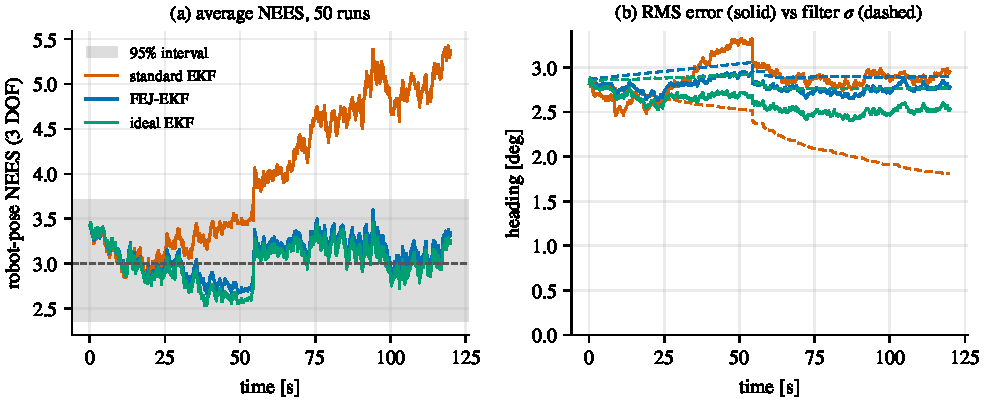
\includegraphics[width=\linewidth]{fig_fej.pdf}
\caption{Planar EKF-SLAM, 50 Monte Carlo runs. (a) Average NEES of the robot pose: the standard EKF leaves the 95\% interval after the first loop
closure (about \SI{55}{s}) and keeps rising, while the FEJ-EKF and the ideal EKF stay consistent. (b) Heading: actual RMS error (solid) and the
filter's own standard deviation (dashed). The initial heading is unobservable, so a consistent, realizable filter keeps reporting about its initial
\SI{2.9}{\degree}, as the FEJ-EKF does. The standard EKF's reported uncertainty falls to \SI{1.8}{\degree} while its actual error stays near \SI{3}{\degree}.}
\label{fig:fej}
\end{figure}

\subsection{A numerical demonstration}

\Cref{fig:fej} compares three filters on the same simulated data (\code{scripts/planar\_sims.py}). A robot drives almost twice around a circle of
radius \SI{10}{m} at \SI{1}{m/s} (\SI{120}{s}), sampling odometry at \SI{10}{Hz} (per-sample noise \SI{0.05}{m/s} in speed and \SI{0.01}{rad/s} in turn
rate), and measures the body-frame position of every landmark within \SI{5}{m} (20 landmarks are scattered around the circle), with \SI{0.1}{m} noise
per axis. The initial pose estimate has \SI{0.1}{m} position and
\SI{0.05}{rad} heading uncertainty. The three filters differ only in where they evaluate their Jacobians:
\begin{itemize}
  \item the \emph{standard EKF} uses the latest estimates, \eqref{eq:slam-phi}--\eqref{eq:slam-H};
  \item the \emph{FEJ-EKF} follows \cref{prop:fej};
  \item the \emph{ideal EKF} evaluates every Jacobian at the true state. It is not realizable, but it is the benchmark for consistency, since its
        linearized model has the true nullspace.
\end{itemize}
The heading panel makes the failure concrete. The initial heading error is unobservable, so no realizable filter can reduce it: the RMS heading
error of the standard and FEJ filters stays near its initial value of about \SI{2.9}{\degree}. (The ideal EKF reduces it slightly, to \SI{2.5}{\degree}, because
its Jacobians are evaluated at the true state, which leaks information that no real filter has.) The FEJ and ideal filters report standard
deviations that match their errors. The standard EKF reports a standard deviation that shrinks steadily, fastest at the loop closure, until its
variance is less than 40\% of its actual mean squared error. It has ``learned'' the global heading from relative measurements, which is impossible. Its NEES grows accordingly, and nothing in its
innovations reveals the problem.

\subsection{FEJ in the MSCKF}

The rule generalizes directly~\cite{li2013msckf2}: \emph{every state appears in the observability matrix at a single linearization point}. Concretely:
\begin{enumerate}
  \item \textbf{Propagation.} The transition matrix from $t_k$ to $t_{k+1}$ is evaluated with the propagated estimates at both ends,
        $\hat x_{k|k-1}$ and $\hat x_{k+1|k}$, wherever it depends on the state (positions, velocities, attitudes). The test is the planar one: the product of
        consecutive transition matrices must telescope.
  \item \textbf{Measurement.} Each clone enters the camera Jacobians at its \emph{first estimate}, the pose it had when it was cloned, not its
        current corrected value. The residual still uses the current value.
  \item \textbf{Feature.} The feature position used in $H_{x,j}$ and $H_{f,j}$ can be any single estimate (for example the triangulation from the
        current clone estimates), because the feature is eliminated: $A_j\T H_{f,j}N_f = 0$ for whatever $N_f$ the chosen value implies.
\end{enumerate}
The precise formulas depend on the error parameterization. For yours, the systematic procedure is: write $N$ in your error coordinates
(\eqref{eq:nullspace-N}), then choose the linearization points so that $\Phi_kN_k = N_{k+1}$ and $H_kN_k = 0$ hold \emph{exactly}, with $N_k$ built from the
first estimates. Even attitude blocks that do not seem to depend on the state may need attention: with a local attitude error, the yaw entry
$\hat R\T e_z$ of $N$ depends on the attitude estimate, so the attitude block of $\Phi_k$ must map $\hat R_{k|k-1}\T e_z$ to $\hat R_{k+1|k}\T e_z$.

\begin{implnote}[storing first estimates without allocation]
FEJ needs, for each clone, a second copy of its pose (the first estimate) next to the current one, and for the IMU state the propagated
estimate of the previous step. Both fit in fixed-size arrays sized by \code{kMaxClones}, so the zero-allocation rules of AGENTS.md E4 are
unaffected. A direct test: on a synthetic run, compute $\|\mathcal{O}N\|$ (or simply $\|H_kN_k\|$ and $\|\Phi_kN_k - N_{k+1}\|$ at every step) for the
standard and the FEJ filter. The FEJ values should be at rounding level, the standard ones visibly larger.
\end{implnote}

% ------------------------------------------------------------------------------
\section{Other remedies}

\subsection{Observability-constrained EKF}
\index{observability-constrained EKF}

Instead of choosing linearization points, the observability-constrained EKF (OC-EKF)~\cite{hesch2014consistency} computes Jacobians at
the latest estimates and then modifies them minimally so that the nullspace conditions hold.

\begin{proposition}[Minimal Jacobian corrections]
\label{prop:oc-ekf}
Let $N_k$ have full column rank. The matrix closest to $H$ in the Frobenius norm that satisfies $H^*N_k = 0$ is
\begin{equation}
  H^* = H\big(I - N_k(N_k\T N_k)\inv N_k\T\big),
\end{equation}
and the matrix closest to $\Phi$ that satisfies $\Phi^*N_k = N_{k+1}$ is
\begin{equation}
  \Phi^* = \Phi + (N_{k+1} - \Phi N_k)(N_k\T N_k)\inv N_k\T .
\end{equation}
\end{proposition}
\begin{proof}
The Frobenius norm is the sum of the squared norms of the rows, and the constraints act on each row separately: row $h$ must satisfy
$h^*N_k = c$ for a given row vector $c$ ($c = 0$ for $H$, a row of $N_{k+1}$ for $\Phi$). Minimizing $\|h^* - h\|^2$ subject to $h^*N_k = c$ is a least-norm problem
for the correction $d = h^* - h$: $dN_k = c - hN_k$. Its minimum-norm solution is $d = (c - hN_k)(N_k\T N_k)\inv N_k\T$ (\cref{sec:least-squares}), which gives both
formulas.
\end{proof}

The OC-EKF thus projects the information along $N$ out of every measurement and enforces the correct propagation of $N$, so the linearized
model has the correct unobservable subspace by construction. The choice of $N_k$ (which estimates to build it from) still matters; Hesch et
al.\ build it from the propagated estimates.

\subsection{Invariant EKF}
\index{invariant EKF}\index{extended pose group}

The invariant EKF~\cite{barrau2017invariant} attacks the root cause: the estimate dependence of $N$. It represents the IMU state as one element
of the \emph{extended pose group} $\mathrm{SE}_2(3)$,
\begin{equation}
  X = \begin{bmatrix} R & v & p \\ 0 & 1 & 0 \\ 0 & 0 & 1 \end{bmatrix} \in \R^{5\times5}, \qquad
  X\inv = \begin{bmatrix} R\T & -R\T v & -R\T p \\ 0 & 1 & 0 \\ 0 & 0 & 1 \end{bmatrix},
\end{equation}
a generalization of $\SE$ (\cref{sec:se3}) with two translation-like columns (features can be appended as further columns), and it defines the
error as the \emph{right-invariant} group error $\eta = \hat XX\inv = \Exp(\xi)$, with $\xi = (\xi_R, \xi_v, \xi_p) \in \R^9$.

\begin{proposition}[Constant unobservable directions]
\label{prop:invariant-nullspace}
In right-invariant error coordinates, the four unobservable directions of \cref{thm:vio-unobservable} are the constant vectors
$\xi = (e_z, 0, 0)$ (yaw) and $\xi = (0, 0, t)$, $t \in \R^3$ (translation), independent of the estimate.
\end{proposition}
\begin{proof}
A global yaw and translation act on the true state from the left: $X \mapsto GX$ with $G = \begin{bmatrix} R_z & 0 & t \\ 0 & 1 & 0 \\ 0 & 0 & 1\end{bmatrix}$, which is
$p \mapsto R_zp + t$, $v \mapsto R_zv$, $R \mapsto R_zR$. The error becomes $\hat X(GX)\inv = \hat XX\inv G\inv = \eta\,G\inv$. For small errors and a small
$G = \Exp(\epsilon)$, with $\epsilon = (\alpha e_z, 0, t)$, the product $\Exp(\xi)\Exp(-\epsilon)$ is $\Exp(\xi - \epsilon)$ to first order. The family of
indistinguishable states therefore differs, in error coordinates, by the constant vectors $\epsilon$.
\end{proof}

Compare \eqref{eq:nullspace-N}, where the yaw direction involves $\hat p$, $\hat v$ and $\hat R$. Because the group structure couples rotation with velocity
and position, a global yaw is a pure rotation error in these coordinates. Two consequences follow. The linearized error dynamics of the IMU (without
biases) are independent of the estimate, $\dot\xi = A\xi + \dots$ with
$A = \begin{bmatrix} 0 & 0 & 0 \\ \sx{g_w} & 0 & 0 \\ 0 & I & 0 \end{bmatrix}$, and $AN = 0$ because $\sx{g_w}e_z = 0$; and since every measurement is invariant under
$X \mapsto GX$, every measurement Jacobian, evaluated at \emph{any} estimate, annihilates the constant $N$. The linearized filter has the correct
unobservable subspace by construction, with no bookkeeping of first estimates. Biases break the exact estimate-independence of the error dynamics,
but not this nullspace property, since $N$ has no bias components. The price is a different state representation, different Jacobians, and a different reset;
it is a deviation from AGENTS.md C3--C4 that this project does not take.

\subsection{Robocentric formulations}
\index{robocentric filter}

A robocentric filter expresses everything relative to the current body frame, so the unobservable global quantities are not estimated at all,
and the global pose is recovered by composing relative motions outside the filter. The nullspace problem disappears with the unobservable states,
at the cost of a more complex propagation in which every state moves when the body moves.

\begin{center}\small
\begin{tabularx}{\linewidth}{@{}l>{\raggedright\arraybackslash}X>{\raggedright\arraybackslash}X@{}}
\toprule
Remedy & What changes & Cost \\
\midrule
FEJ & linearization points of $\Phi$ and $H$ & store first estimates; slightly larger linearization error \\
OC-EKF & Jacobians projected onto the constraint & build $N_k$ each step; extra products \\
Invariant EKF & state representation and error definition & new derivations; leaves the frozen conventions \\
Robocentric & state is relative to the body & more complex propagation \\
\bottomrule
\end{tabularx}
\end{center}

% ------------------------------------------------------------------------------
\section{Degenerate motions}
\index{degenerate motions}

\Cref{thm:vio-unobservable} assumes \emph{general} motion. Some motions remove further directions~\cite{yang2019degenerate}.
\begin{center}\small
\begin{tabular}{@{}l l@{}}
\toprule
Motion & What becomes unobservable \\
\midrule
constant velocity (no acceleration) & metric scale \\
pure rotation (no translation) & feature depths and translation scale \\
no rotation & accelerometer bias inseparable from the gravity direction (tilt) \\
at rest & both of the above, plus everything that needs parallax \\
\bottomrule
\end{tabular}
\end{center}
Each row has a short explanation. At constant velocity the accelerometer measures only gravity and bias, so nothing ties the size of the
camera's (scale-free) motion estimate to meters. Without translation there is no parallax, so depths, and with them the scale of the
translation, cannot be triangulated. Without rotation the gravity direction in the body frame is constant, and a constant error in it is
indistinguishable from a constant accelerometer bias; rotation makes gravity sweep through the body axes while the bias stays fixed, which
separates them.

The filter does not fail during such motions, provided it is consistent: its covariance simply stops shrinking along the
affected directions until informative motion returns. An inconsistent filter, by contrast, may ``learn'' these quantities from
noise. When a vehicle is known to be stationary, a \emph{zero-velocity update} (the pseudo-measurement $v = 0$, \cref{ch:updates}) supplies real
information and stops drift, which is why many systems detect stillness explicitly.

\begin{takeaways}
\begin{itemize}
  \item The unobservable subspace is the nullspace of the observability matrix; a filter must not gain information along it. For nonlinear
        systems, the gradients of the output's Lie derivatives play the role of the observability matrix.
  \item VIO has four unobservable directions: global translation and rotation about gravity. Roll, pitch and scale are observable
        under general motion.
  \item In local error coordinates the yaw direction is $\hat R\T e_z$ for the attitude and $-\sx{\hat p}e_z$ for positions: it depends on
        the estimate.
  \item Linearizing the same state at different estimates makes the global heading spuriously observable: in planar SLAM the leak is
        $\hat R_k\T\Omega(D_k + \bar\ell_j - \hat\ell_j)$, driven by the accumulated corrections and the drift of the landmark estimates.
  \item FEJ restores the nullspace by fixing each state's linearization point; OC-EKF projects the Jacobians; the invariant EKF makes the
        unobservable directions constant; degenerate motions remove further directions.
\end{itemize}
\end{takeaways}

\begin{exercises}
  \item Verify \eqref{eq:nullspace-N} numerically: apply a small yaw rotation and translation to a random state and compute
        $x'\bminus x$.
  \item Show that the translation columns of $N$ remain in the nullspace of the EKF's observability matrix even when Jacobians are
        evaluated at changing estimates.
  \item Redo the worked example on Lie derivatives with two unknown landmarks. What is the rank of $d\mathcal{O}$, and what are the unobservable
        directions?
  \item Repeat \cref{thm:slam-obs} for range-and-bearing measurements, $z = (\|d\|, \atantwo(d_y, d_x))$ with $d = R(\psi)\T(\ell_j - p)$. Show that the leak
        has the same form.
  \item Modify \code{scripts/planar\_sims.py} to print $\|H_k\Phi_{k-1}\cdots\Phi_1N\|$ for the three filters of \cref{fig:fej}, and confirm that only the
        standard EKF violates the nullspace condition.
  \item Prove that the minimum-norm solution used in \cref{prop:oc-ekf} is indeed the minimizer, by writing $d = d_\parallel + d_\perp$ with $d_\parallel$ in the row space of
        $N_k\T$.
  \item Implement a zero-velocity update as an EKF measurement and derive its $H$. When is it safe to apply?
  \item Read~\cite{li2013msckf2} and list which Jacobians must be evaluated at first estimates in the MSCKF. Sketch how you would store
        the first estimates in the project's data structures without allocation.
\end{exercises}
